%%% Local Variables: 
%%% coding: utf-8
%%% mode: latex
%%% TeX-engine: xetex
%%% End: 

\documentclass[hide notes,intlimits]{beamer}

\mode<presentation>
{
  \usetheme[footline]{PISMshade}
  \setbeamercovered{transparent}
}

% load packages
\usepackage{media9}
\usepackage[english]{babel}
\usepackage[multidot]{grffile}

\usepackage{tikz}
\usetikzlibrary{shapes,arrows}
\usetikzlibrary{shadows}

\definecolor{dark red}{HTML}{E41A1C}
\definecolor{dark green}{HTML}{4DAF4A}
\definecolor{dark violet}{HTML}{984EA3}
\definecolor{dark blue}{HTML}{084594}
\definecolor{dark orange}{HTML}{FF7F00}
\definecolor{light blue}{HTML}{377EB8}
\definecolor{light red}{HTML}{FB9A99}
\definecolor{light violet}{HTML}{CAB2D6}

\setbeamercolor{boxed}{fg=black,bg=light blue!25}
\graphicspath{{figures/}{../figures/}{../figures_2018_08/}{../2021_09_cph/figures/}}

\newenvironment{transbox}[1][]{%
\begin{tikzpicture}
\node[drop shadow,rounded corners,text width=.9\textwidth,fill=white, fill opacity=#1,text opacity=1] \bgroup
}{
\egroup;\end{tikzpicture}} 

\newenvironment{transbox-tight}{%
\begin{tikzpicture}
\node[drop shadow,rounded corners,fill=uaf yellow, fill opacity=0.75,text opacity=1] \bgroup
}{
\egroup;\end{tikzpicture}} 

\newcommand{\jl}{[\![}
\newcommand{\jr}{]\!\hskip 0.003cm ]}
\newcommand{\bpsi}{\boldsymbol{\psi}}
\newcommand{\bPsi}{\boldsymbol{\Psi}}
\newcommand{\bphi}{\boldsymbol{\phi}}
\newcommand{\bPhi}{\boldsymbol{\Phi}}
\newcommand{\bn}{\mathbf{n}}
\newcommand{\bq}{\mathbf{q}}
\newcommand{\bv}{\mathbf{v}}
\newcommand{\D}{\,\mathrm{d}}
\newcommand{\Tsnow}{T_{\text{snow}}}
\newcommand{\Hatm}{H_{\text l}^{\text{atm}}}

\newcommand{\mathtext}[1]{\mathsf{#1}}

% title page
\title[Ice sheet modeling] % (optional, use only with long paper titles)
{Towards credible projections of sea-level rise}

\author[Aschwanden] % (optional, use only with lots of authors)
{\textbf{Andy Aschwanden}\\ with \\D. Brinkerhoff, M. Truffer, T. Bartholomaus}
\institute{Geophysical Institute, University of Alaska Fairbanks}

% - Give the names in the same order as the appear in the paper.
% - Use the \inst{?} command only if the authors have different
%   affiliation.

% - Use the \inst command only if there are several affiliations.
% - Keep it simple, no one is interested in your street address.
 \titlegraphic{\vskip-.5cm\includegraphics[height=1.5cm]{pism_logo_v2_transp}}

\date{}


\subject{The Greenland Ice Sheet}

\begin{document}



\setbeamertemplate{background canvas}
  {
     \tikz{\node[inner sep=0pt,opacity=0.6] {\includegraphics[height=\paperheight]{earth-drowning-desat}};}
}


 
% insert titlepage
\begin{frame}
  \titlepage
  \note[item]{Collaboration Martin, Doug, Tim}
\end{frame}


\setbeamertemplate{background canvas}
  {
     \tikz{\node[inner sep=0pt,opacity=0.35] {\includegraphics[height=\paperheight]{earth-drowning-desat}};}
}


\part{A little ice sheet modeling history}

\frame{\partpage}


\begin{frame}{Modern sea-level change}
  \vspace{-1.5em}
  \begin{minipage}[t][5cm][t]{\textwidth}
    \begin{figure}
      \includegraphics<1->[height=5cm]{sea-level-from-altimetry}\\
    \end{figure}
  \end{minipage}
  \vspace{-2.em}
  \begin{minipage}[t][4cm][t]{\textwidth}
  \begin{columns}[c]
    \begin{column}{.45\textwidth}
      \uncover<1>{Sea-level contribution 1993--18}
      \uncover<2>{Sea-level contribution 2006--18}
    \end{column}
    \begin{column}{.45\textwidth}
    \includegraphics<1>[height=2.75cm]{sea-level-contrib-1993-2018}
    \includegraphics<2>[height=2.75cm]{sea-level-contrib-2006-2018}
    \end{column}
  \end{columns}
  \end{minipage}
\end{frame}

\setbeamertemplate{background canvas}
{
%
}


\begin{frame}
  \frametitle{IPCC AR4, 2007}
  \begin{columns}[c]
    \begin{column}{.4\linewidth}
      \begin{figure}
        \includegraphics[height=5cm]{ar4-wg1}
      \end{figure}
    \end{column}
    \begin{column}{.5\linewidth}
      \begin{figure}
        \includegraphics[height=3.5cm]{no-ice-sheet-models}
      \end{figure}
      \begin{itemize}
      \item No results from ice sheet models included due to the models' inability to track recent changes
      \end{itemize}
    \end{column}
\end{columns}
\end{frame}




\begin{frame}{Observed vs simulated flow speeds (2007 model)}
  \begin{columns}[c]
    \begin{column}{.6\linewidth}
    \begin{figure}
      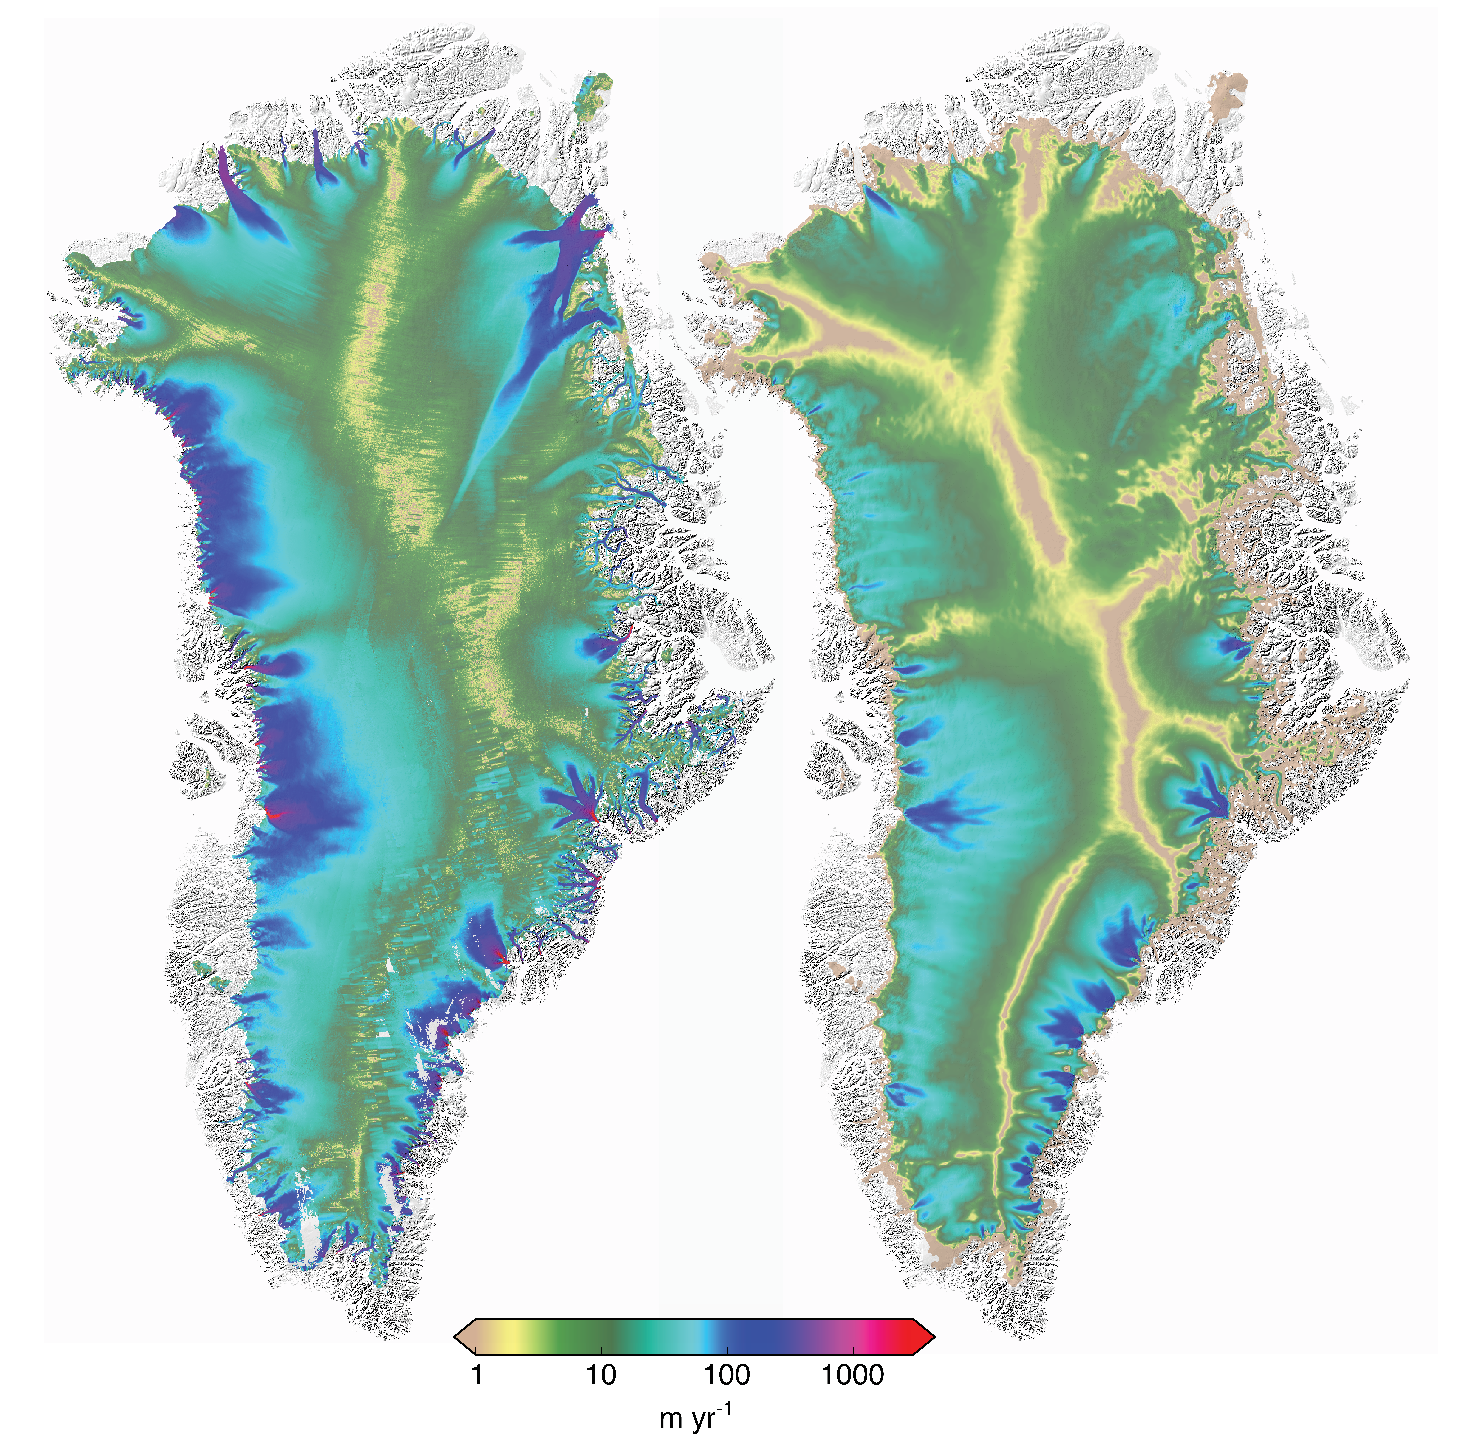
\includegraphics[height=5.75cm]{gris-obs-exp-old}
      \\ \tiny{adapted from Aschwanden, Fahnestock, Truffer (2016) \textit{Nature Comms.}}
    \end{figure}
    \end{column}
    \begin{column}{.4\linewidth}
      \begin{figure}
        \includegraphics[width=.75\textwidth]{roadblocks}
      \end{figure}
      \begin{itemize}
      \item can't reproduce the velocity field
      \item this led to a model development frenzy
      \end{itemize}
    \end{column}
  \end{columns}
  \note[item]{}
\end{frame}


\begin{frame}
  \frametitle{IPCC AR5, 2013}
  \begin{columns}[c]
    \begin{column}{.4\linewidth}
      \begin{figure}
        \includegraphics[height=5cm]{ar5-wg1}
      \end{figure}
    \end{column}
    \begin{column}{.6\linewidth}
      \begin{figure}
        \includegraphics[width=4.75cm]{searise}
      \end{figure}
      \begin{figure}
        \includegraphics[width=4.75cm]{nick2013}
      \end{figure}
    \end{column}
  \end{columns}
\end{frame}

\begin{frame}{Observed vs simulated flow speeds (2013 model)}
  \alert{Have the models gotten any better? Not really.}
  \begin{columns}[c]
    \begin{column}{.6\linewidth}
    \begin{figure}
      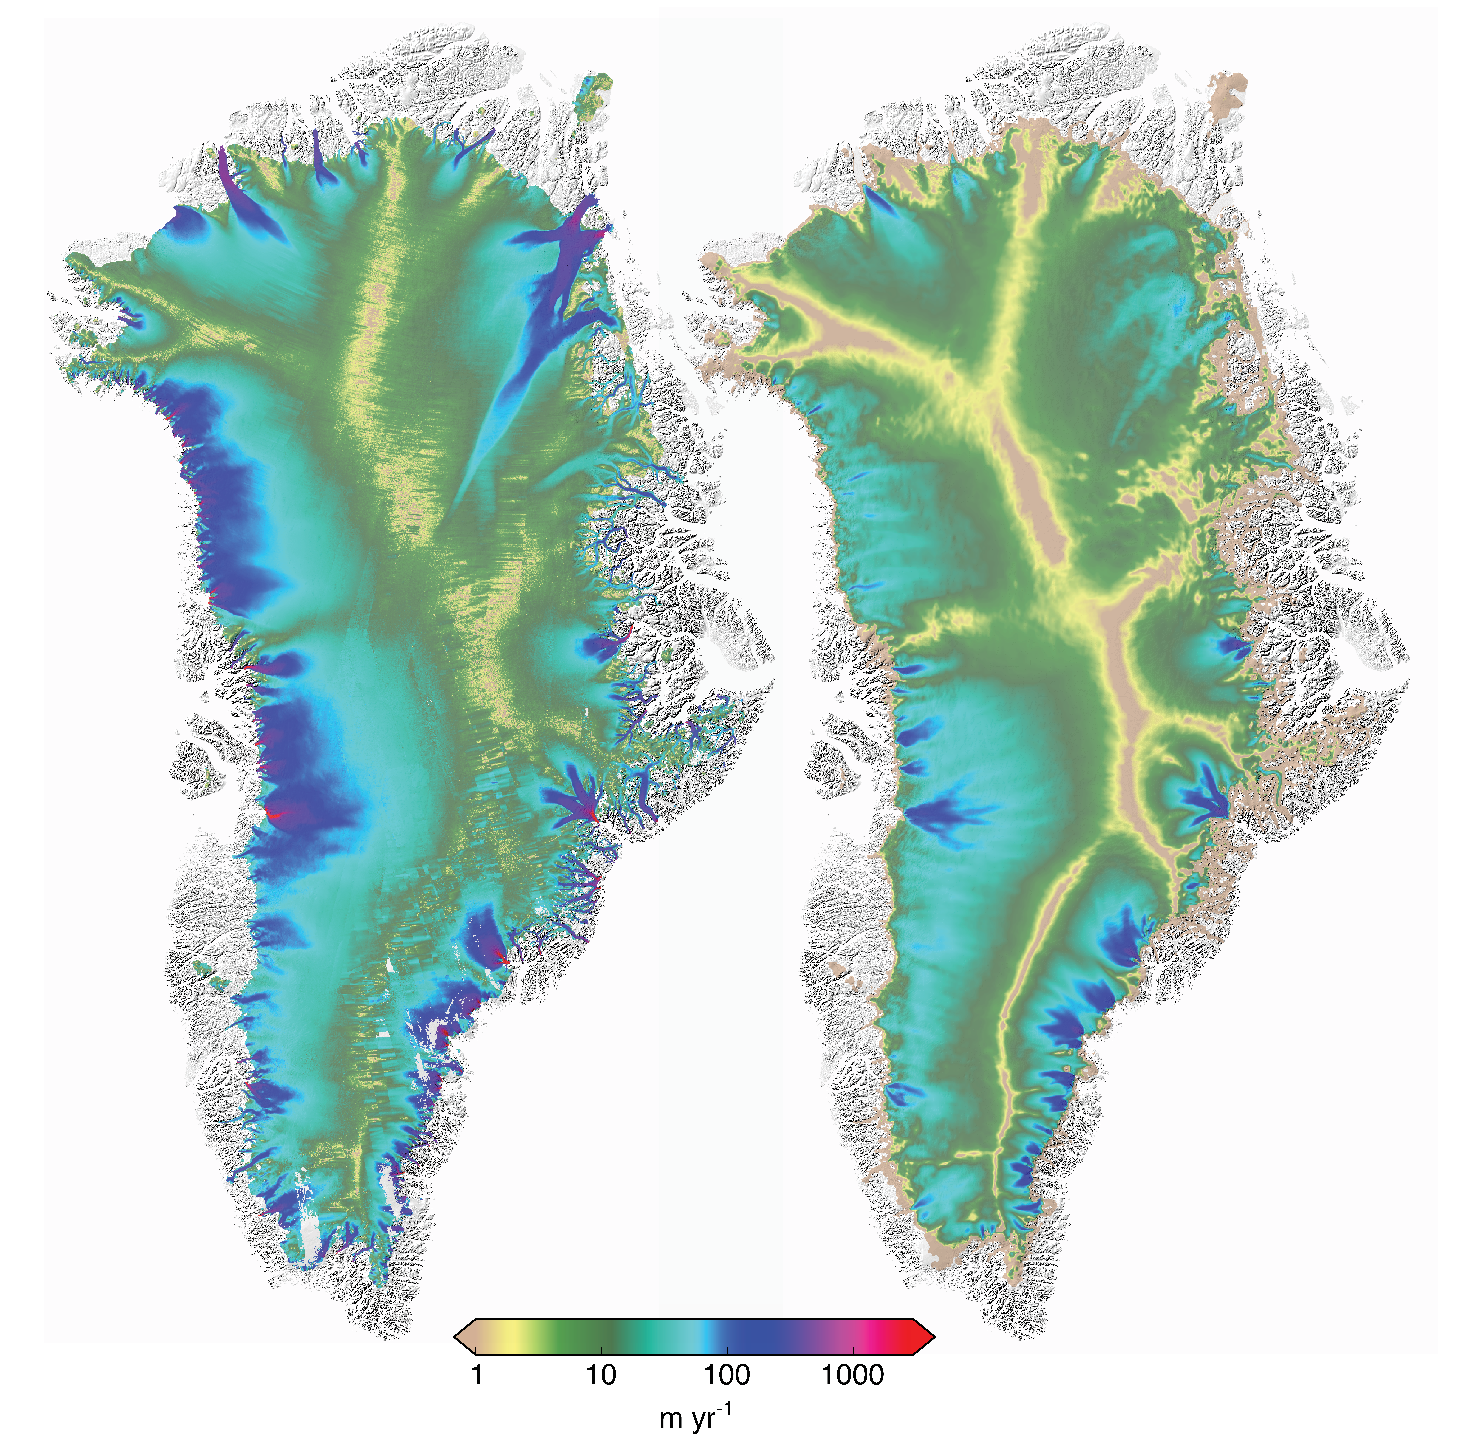
\includegraphics[height=5.75cm]{gris-obs-exp-old}
      \\ \tiny{adapted from Aschwanden, Fahnestock, Truffer (2016) \textit{Nature Comms.}}
    \end{figure}
    \end{column}
    \begin{column}{.4\linewidth}
      \begin{figure}
        \includegraphics[width=.75\textwidth]{roadblocks}
      \end{figure}
      \begin{itemize}
      \item still can't reproduce the velocity field
      \end{itemize}
    \end{column}
  \end{columns}
  \note[item]{}
\end{frame}




\begin{frame}{Post 2014 models}
  \alert{Have the models gotten any better? Yes. Sort of.}
  \begin{columns}[c]
    \begin{column}{.6\linewidth}
    \begin{figure}
      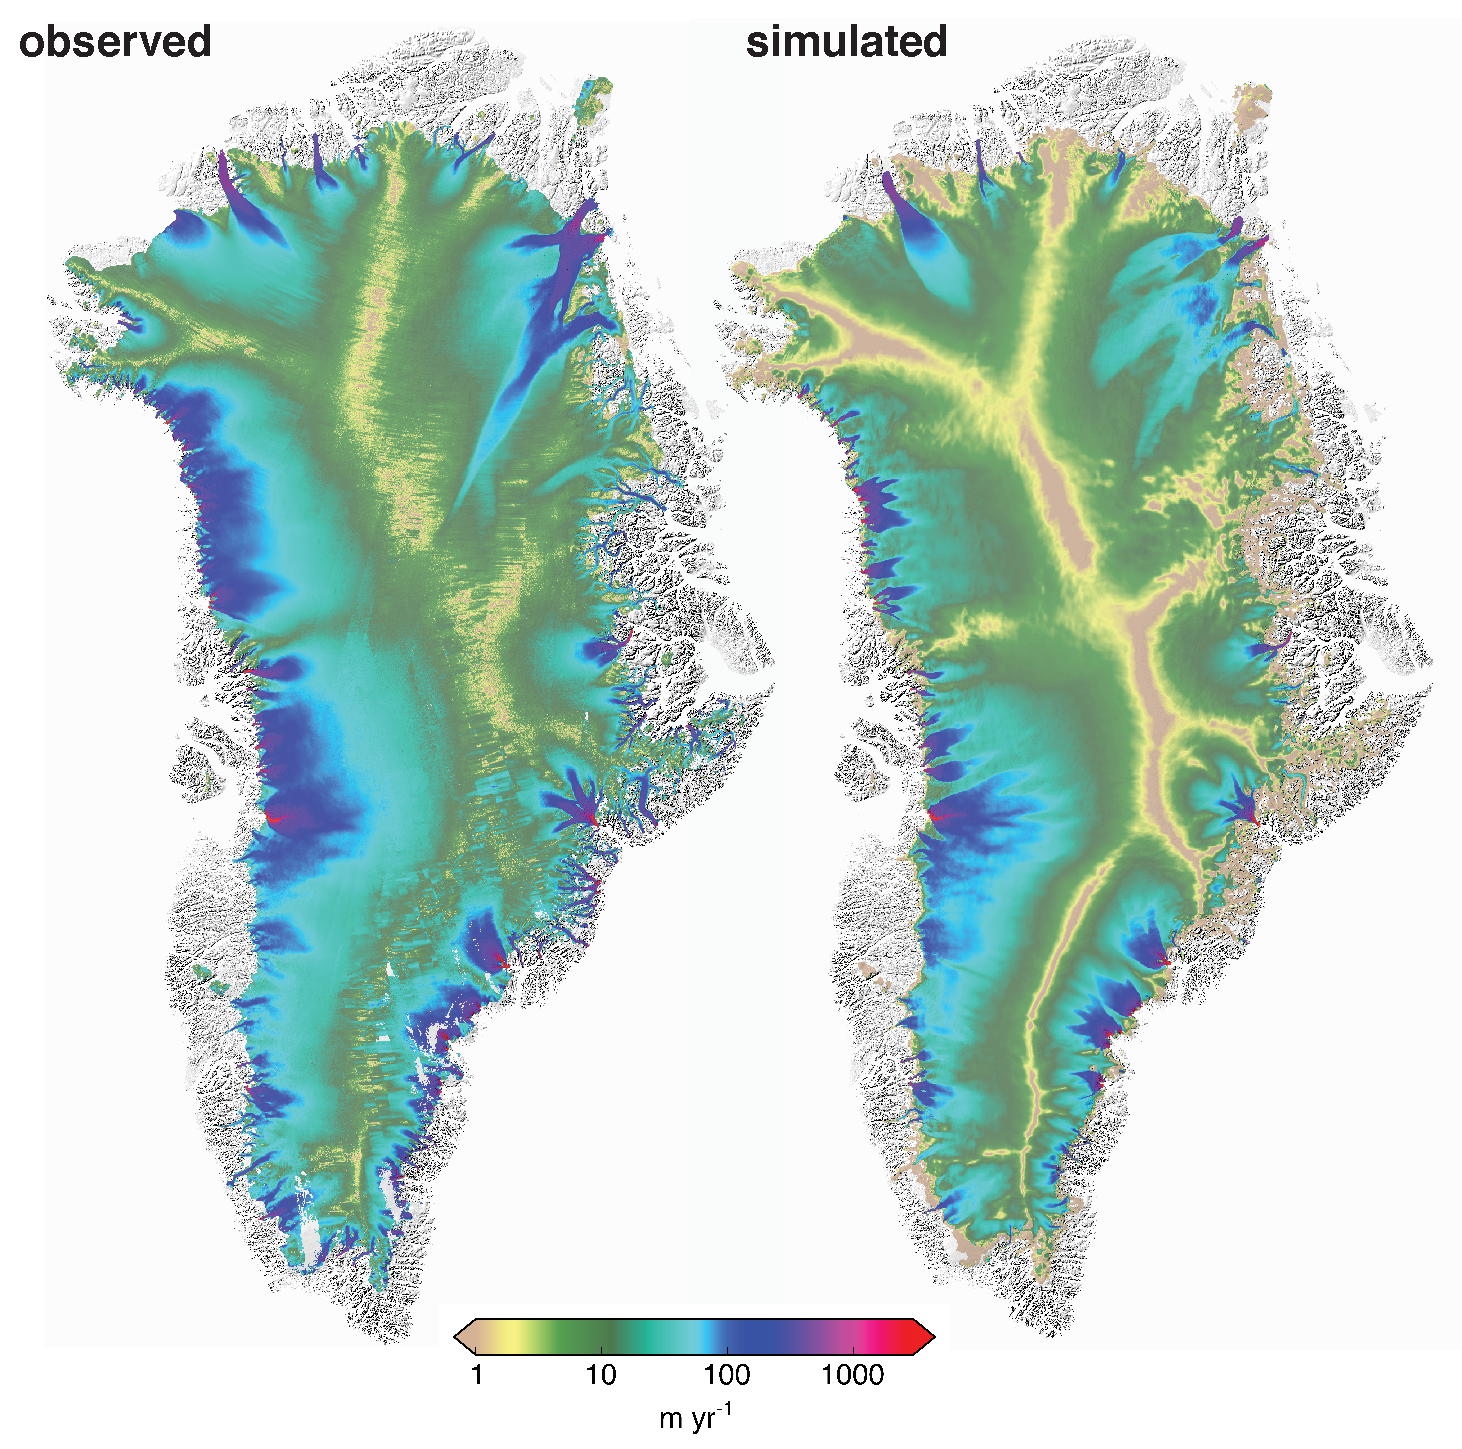
\includegraphics[height=5.75cm]{gris-obs-exp-new}
      \\ \tiny{adapted from Aschwanden, Fahnestock, Truffer (2016) \textit{Nature Comms.}}
    \end{figure}
    \end{column}
    \begin{column}{.4\linewidth}
      \begin{figure}
        % \includegraphics[height=1cm]{oib} \\
        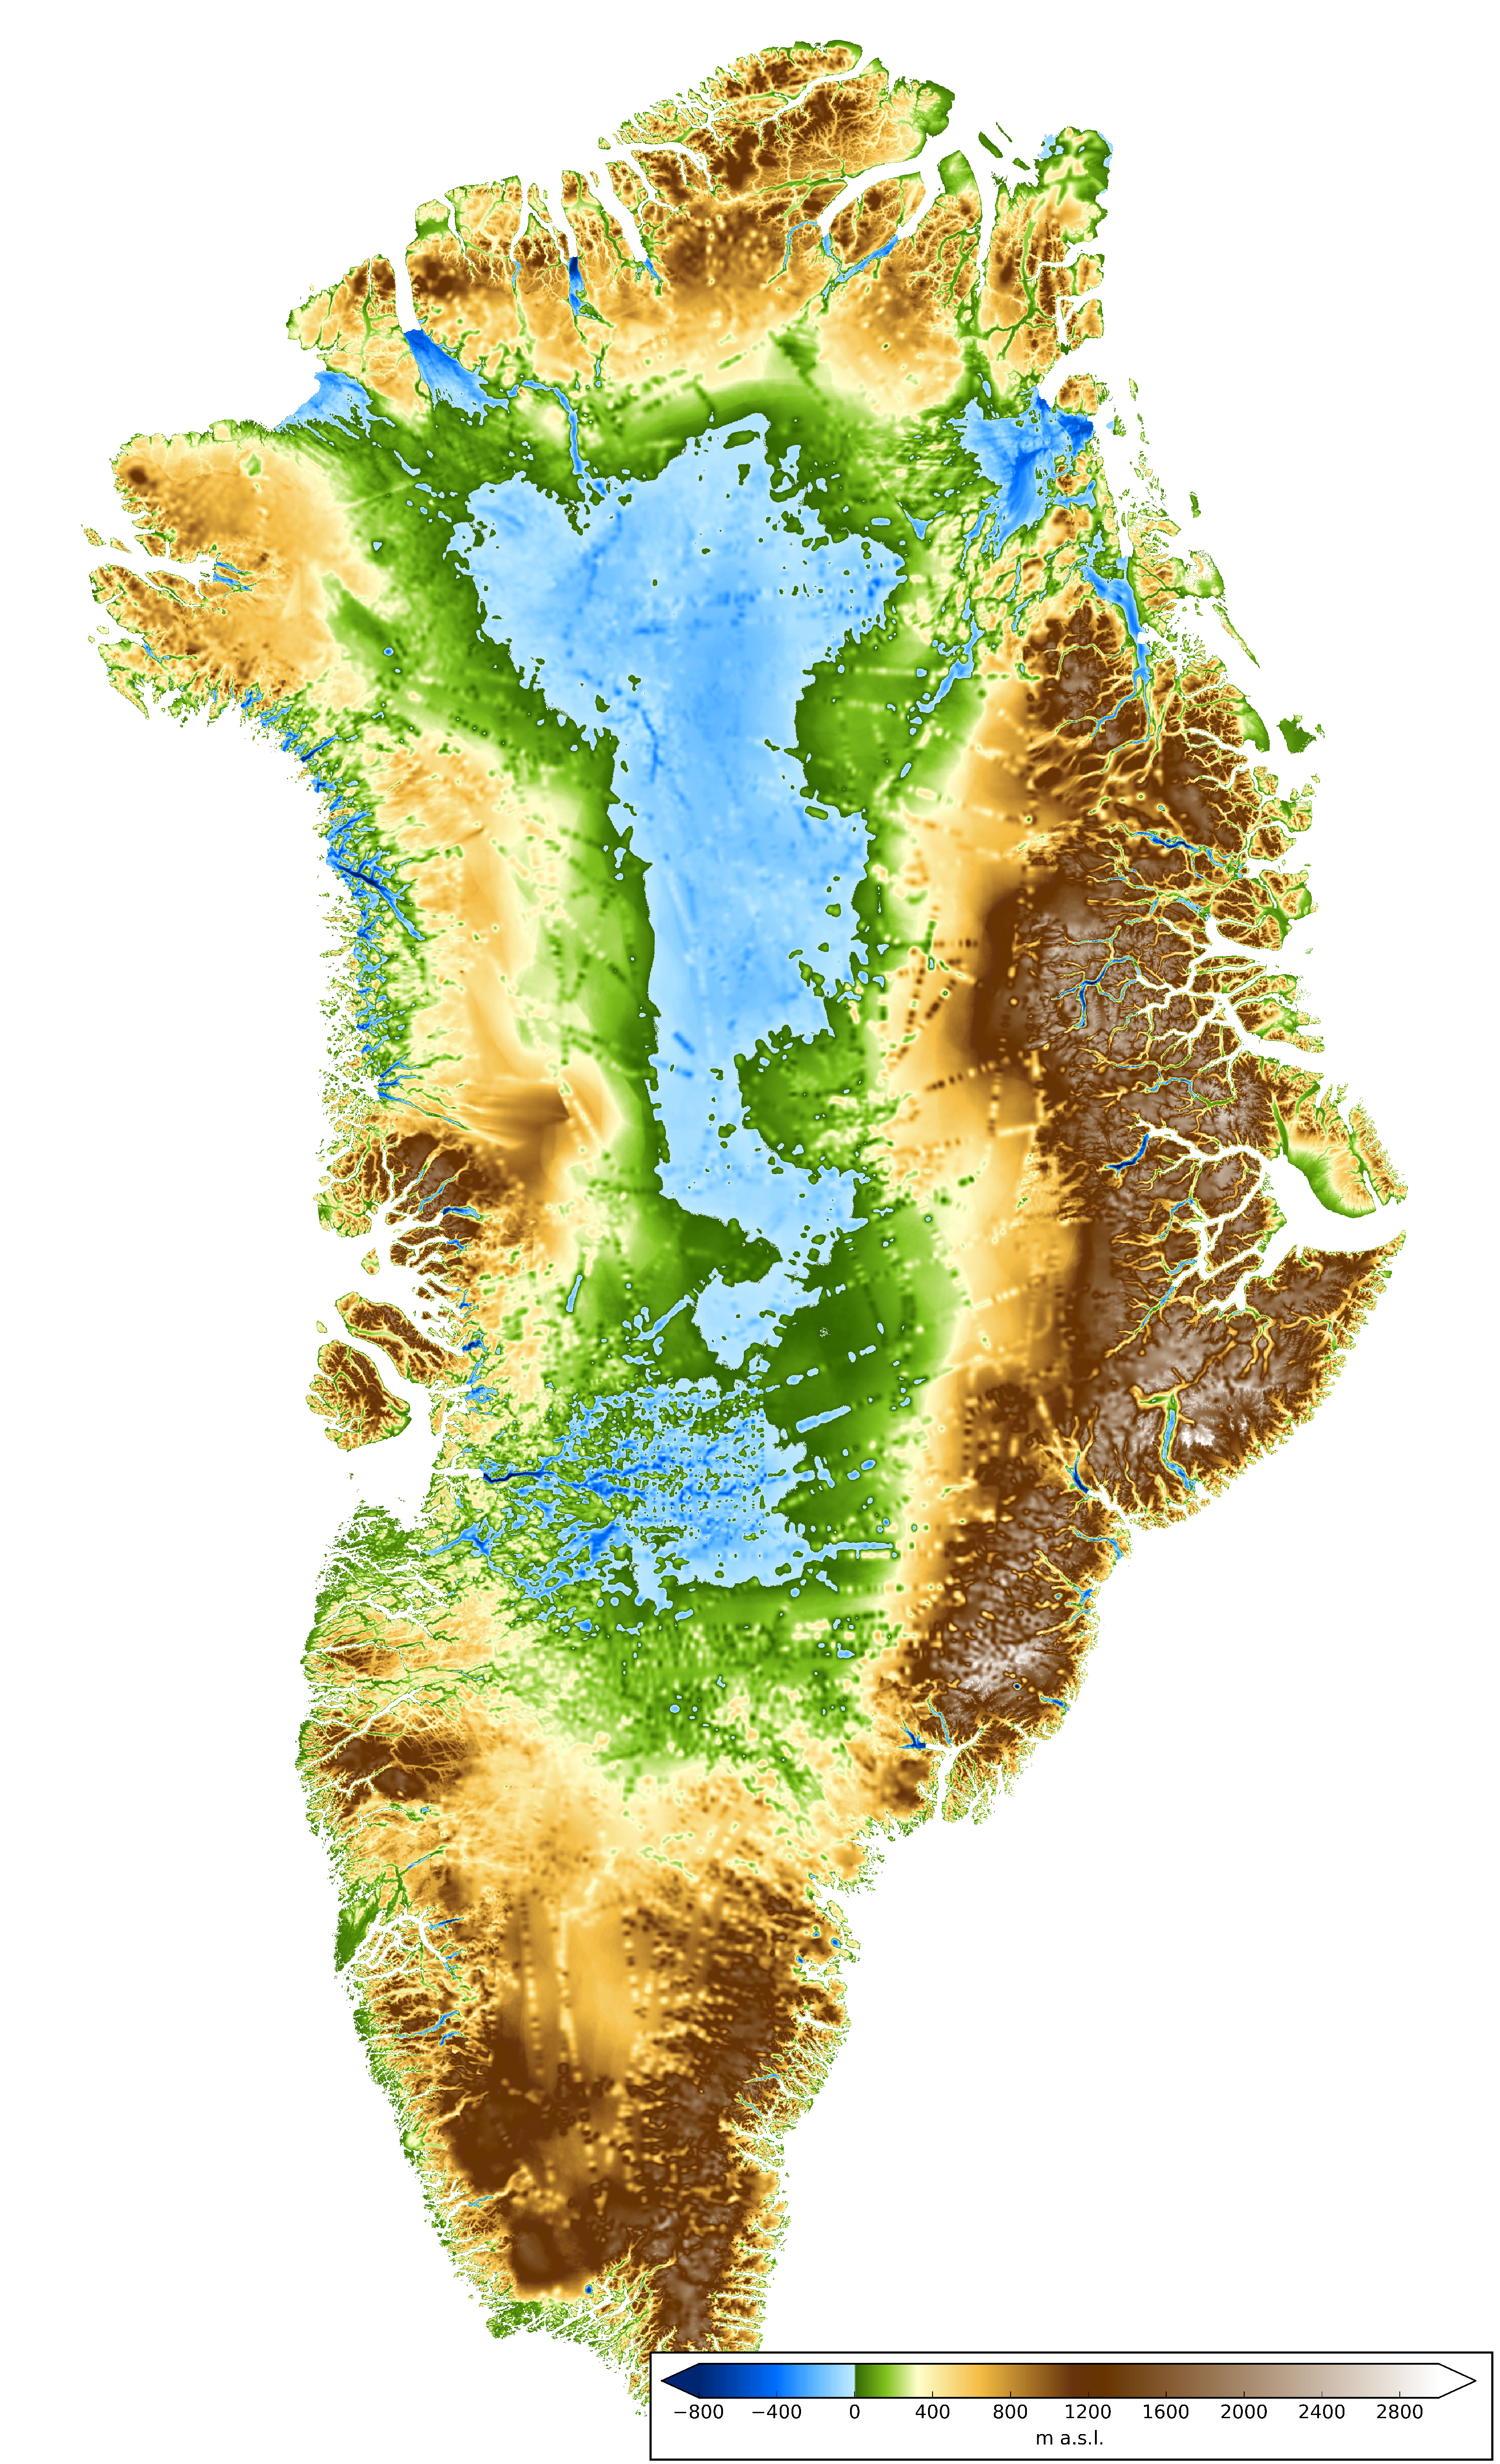
\includegraphics[height=5.75cm]{greenland-bed-mcb}
      \\ \tiny{adapted from Morlighem et al. (2014) \textit{Nature Geosci.}}
      \end{figure}
    \end{column}
  \end{columns}
  \alert{Accurate ice thickness does the trick}
  
  \note[item]{first time capturing the flow field for the right reason}
  \note[item]{this is quite a break through in ice sheet modeling}
  \note[item]{though not a surprising one}
  \note[item]{it just confirms what students learn in glaciology 100:}
  \note[item]{ice flows downhill}
\end{frame}


\begin{frame}
  \frametitle{IPCC AR6, 2021}
  \begin{columns}[c]
    \begin{column}{.4\linewidth}
      \begin{figure}
        \includegraphics[height=5cm]{ar6-wg1}
      \end{figure}
    \end{column}
    \begin{column}{.6\linewidth}
      \begin{itemize}
      \item multi-model ensemble
      \item Ice Sheet Model Intercomparison Project for CMIP6 (ISMIP6)
        \includegraphics<1>[width=2cm]{ismip6_logo}
      \end{itemize}
    \end{column}
  \end{columns}
\end{frame}



\begin{frame}{Modern and projected mass loss from Greenland}
  \begin{figure}
    \includegraphics<1>[width=3cm]{ismip6_logo}
  \end{figure}
  \begin{figure}
    \includegraphics<1>[width=.9\textwidth]{ar6-fig17-no-zoom}
    \caption{IPCC AR6, Fig. 9.17}
  \end{figure}
\end{frame}

\begin{frame}{All sunshine and rainbows?}
  \begin{figure}
    \includegraphics<1->[width=.75\textwidth]{sunshine_rainbows}
  \end{figure}
  \uncover<2>{\alert{What a minute\ldots}}
\end{frame}

\begin{frame}{Modern and projected mass loss from Greenland II}
  \begin{figure}
    \includegraphics<1>[width=.9\textwidth]{ar6-fig17-no-zoom}
    \includegraphics<2>[width=.9\textwidth]{ar6-fig17-with-zoom}
    \caption{IPCC AR6, Fig. 9.17}
  \end{figure}
\end{frame}


\begin{frame}{A closer look}
  \begin{figure}
    \includegraphics[width=\textwidth]{GIS_hist_with_obs}
    \caption{Aschwanden, Brinkerhoff, Bartholomaus, \& Truffer (in press)}
  \end{figure}
  \begin{columns}[c]
    \begin{column}{.5\textwidth}
      \begin{minipage}[t][.5\textheight][t]{\textwidth}
        \alert{Almost all historical simulations under-estimate modern mass loss}
      \end{minipage}
    \end{column}
    \begin{column}{.25\textwidth}
      \begin{minipage}[t][.5\textheight][t]{\textwidth}
        \begin{figure}
          \includegraphics<2>[width=1.8cm]{brain_thinking}
        \end{figure}
      \end{minipage}
    \end{column}
  \end{columns}
\end{frame}



\begin{frame}{Modern and projected Arctic sea ice extend}
  \vspace{-1em}
  \begin{minipage}[t][1.25cm][t]{\textwidth}
    \begin{figure}
      \includegraphics<1->[width=1cm]{brain_solution}
    \end{figure}
  \end{minipage}
  \vspace{0.25em}
  \begin{minipage}[t][6.75cm][b]{\textwidth}
    \begin{figure}
      \includegraphics<2>[height=5.5cm]{grl23061-fig-0001}
    \end{figure}
  \end{minipage}
\end{frame}


\setbeamertemplate{background canvas}
  {
     \tikz{\node[inner sep=0pt,opacity=0.35] {\includegraphics[height=\paperheight]{earth-drowning-desat}};}
}


\part{A way forward}

\frame{\partpage}

\setbeamertemplate{background canvas}
  {
}

\begin{frame}{2 key requirements}
Accurate predictions of the cryosphere's contribution to sea level require that models:
\begin{enumerate}
    \item<1> Fully characterize uncertainties in model structure, parameters, initial conditions, and boundary conditions.
    \item<1-2> Yield simulations that fit observations within observational uncertainty. 
\end{enumerate}
  \begin{figure}
    \includegraphics[width=0.45\textwidth]{difference-accuracy-and-precision}
  \end{figure}
\end{frame}

\begin{frame}{The first large ensemble projections for Greenland}
  \begin{figure}
    \includegraphics[width=0.8\textwidth]{Greenland_RCP_85_2008_2300_comp_4k.0293_print}
    \caption{NASA Scientific Visualization Studio. After Aschwanden et al. (2019).}
  \end{figure}
\end{frame}


\begin{frame}{AS19 Ensemble Projections}
  \begin{minipage}[t][4cm][t]{\textwidth}
    \begin{figure}
      \includegraphics[height=4cm]{projection_as19_bars}
    \end{figure}
  \end{minipage}
  \alert{Prescribe pior distributions to assess parametric uncertainty}
  \begin{minipage}[t][3cm][t]{\textwidth}
    \begin{figure}
      \includegraphics[height=3cm]{prior}
    \end{figure}
  \end{minipage}
\end{frame}



\begin{frame}{What's wrong with AS19}
  \begin{minipage}[t][4cm][t]{\textwidth}
    \begin{figure}
      \includegraphics[height=4cm]{projection_as19_bars}
    \end{figure}
  \end{minipage}
  \alert{No conditioning on observations}
  \begin{minipage}[t][3cm][t]{\textwidth}
  \end{minipage}
\end{frame}

\begin{frame}{A Bayesian (Probabilistic) Calibration in two steps}
    \begin{minipage}[t][2cm][t]{\textwidth}
      \begin{block}{Which observations should we use?}
        \begin{itemize}
        \item<1-> use the quantity of interest: mass change
        \item<2> use quantity that contributes a lot to uncertainty: ice flow
        \end{itemize}
        \note[item]{}
      \end{block}
  \end{minipage}
    \begin{minipage}[t][6cm][t]{\textwidth}
        \begin{columns}[c]
    \begin{column}{.3\textwidth}
    \includegraphics<1->[height=5.5cm]{greenland-obs-rignot}
    \end{column}
    \begin{column}{.65\textwidth}
    \includegraphics<2>[height=3cm]{GIS_hist_only_obs}
    \end{column}
  \end{columns}

    \end{minipage}

\end{frame}


\begin{frame}{1. Ice Flow calibration: strategy}
\begin{itemize}
\item use Markov Chain Monte Carlo sampling to find the joint distribution of these parameters given observations.
\item think of PISM as a map $\mathcal{F}$ from a parameter vector $\mathbf{x}$ to surface speeds $\mathbf{Y}$
\begin{equation}
\mathbf{Y} = \mathcal{F}(\mathbf{x})
\end{equation}
\item running the forward model (PISM) is too expensive for MCMC
\item Generate a ``cheap'' surrogate model $\mathcal{G}$ such that
\begin{equation}
\mathcal{G}(\mathbf{x}) \approx \mathcal{F}(\mathbf{x})
\end{equation}
\end{itemize}

  \note[item]{We take a Bayesian approach and use Markov Chain Monte Carlo sampling to find the joint distribution of these parameters.  While this problem is computationally challenging due to the significant expense of running the forward model, we made it tractable by employing a neural-network based surrogate model that provides a low-cost mapping from parameters to velocity fields \citep{Brinkerhoff2020}.}
\end{frame}

\begin{frame}{1. Ice Flow calibration: surrogate model}

  \begin{figure}
    \includegraphics<1->[width=.5\textwidth]{neural-network}
  \end{figure}
\begin{itemize}
\item use 4 layer Neural Network surrogate model by Brinkerhoff et al (2021)
\item implemented in PyTorch
\item train surrogate model on NVIDIA GPU
\end{itemize}
\end{frame}


\begin{frame}{1. Ice Flow calibration: dimensionality reduction}
  \alert{Challenge $\mathbf{Y}$ is not a scalar}
 $\mathbf{Y}$ is \alert{not} a scalar:
\begin{eqnarray}
\mathbf{x} = \{x_1, x_2,\ldots,x_n\}, & n = 8, \\ 
\mathbf{Y} = \{Y_1, Y_2, \ldots,Y_m \},& m \ge 10^6
\end{eqnarray}
\begin{block}{Doug's genius}
\begin{itemize}
\item decompose training data into ``eigen-glaciers'' using Pricipal Component Analysis (``eigen faces'' in picture analysis)
\item we only need to simulate the first $\sim$100 eigen-coefficients to capture 99.95\% of the variance
\item we have reduced the problem from 10$^6$ to $\sim$100 unknowns.
\end{itemize}
\end{block}
\begin{figure}
  \includegraphics<1->[height=4cm]{eigenglaciers_0}
\end{figure}
\end{frame}


\begin{frame}{1. Ice Flow calibration: training data}
  \begin{figure}
    \includegraphics<1->[width=\textwidth]{prior}
  \end{figure}
\begin{itemize}
\item select 8 relevant parameters
\item define a prior probability distribution for each parameter
\item draw 1,000 samples using Sobol Sequences
\item run PISM 1,000 times
\end{itemize}
\end{frame}




\begin{frame}{1. Ice Flow: Surrogate model}
  \begin{figure}
    \includegraphics<1>[width=0.75\textwidth]{prior}
    \includegraphics<2>[width=0.75\textwidth]{prior_posterior}
  \end{figure}
  \begin{itemize}
  \item using the surrogate model, create 1,000,000 member strong ensemble
  \item run MCMC sampling given observations
  \item what you get are posterior distributions of the parameters
  \item these distributions best fit the surface speeds observations
  \end{itemize}
\end{frame}

\begin{frame}{Use posterior as new prior}
  \begin{minipage}[t][4cm][t]{\textwidth}
  \begin{figure}
    \includegraphics<3->[height=4cm]{projection_flow_bars}
  \end{figure}
  \end{minipage}
  \begin{itemize}
  \item<1-> create 500 samples from posterior
  \item<2-> rerun PISM 500x, wait
  \item<3-> get new projections conditioned on surface speeds
  \item<4-> find reduced variance
  \end{itemize}
\end{frame}

\begin{frame}{2. Mass Loss: Bayesian Calibration}
  \begin{minipage}[t][4cm][t]{\textwidth}
    \begin{figure}
      \includegraphics<3->[height=4cm]{projection_flowmass_bars}
    \end{figure}
  \end{minipage}
  \begin{itemize}
  \item<1->  weight members based on their likelihood relative to observations of mass change.
  \item<2-> resample simulations proportionally to these likelihoods to create a new ensemble that is consistent with respect to both  observations of surface speed and mass change to within observational uncertainty
  \item<3-> get new projections conditioned on surface speeds and mass loss
  \item<4-> find further reduced variance
  \end{itemize}
\end{frame}

\begin{frame}{Putting it together}
  \begin{figure}
    \includegraphics<1>[height=4cm]{projection_as19_bars}
    \includegraphics<2>[height=4cm]{projection_flow_bars}
    \includegraphics<3>[height=4cm]{projection_flowmass_bars}
  \end{figure}
\end{frame}

\begin{frame}{Final thoughts}
  \begin{itemize}
  \item the surrogate model is only used to aid in model calibration
  \item \alert{not} for the actual projections
  \end{itemize}
\end{frame}


\end{document}
